\chapter{Seiyuu Social Network}
Social networks consist of a finite set of actors and the relations between them. Usually represented as a graph; with actors or organizations as set of nodes and a defined relation between them as set of edges. This structures are useful to analyze complex social interactions and communities.

\section{Node and edge definitions}
This social network is of a particular kind called \textit{two-mode networks} which consists of a set of actors (seiyuu) and events (anime). So there exists two ways of viewing it, one will be from seiyuu perspective, using anime in common for edges; the other being from anime perspective, using seiyuu in common for edges. We chose the former since we found more interesting they being actual people and using other information about them such as debut and gender.

So our social network consists of voice actors as nodes and co-workership between them as edges. It's important to notice that this social network is time dependant since each seiyuu has a debut year and each anime has an aired time; giving us freedom to choose different time frames to observe.

Aside from being time dependant there exists different possible definitions of relationship or co-workership between seiyuu. One could say two actors know each other if they have worked in at least one job together, or maybe it requires more than one. There's also a time frame to define, relationship could take into account all works of both of them or only from certain years.\\

\section{Construction}
As a first approach Gephi was used to build the network. Since the graph was big enough to bring performance problems and we needed to build the edges dynamically (which couldn't be done in Gephi) NetworkX was used instead.

NetworkX was chosen because it's an easy yet powerful Python library, it doesn't get along with massive graphs but ours was not big enough to present a problem. 

One can export the graph and open it on Gephi, for a more visual analysis.

And also we needed to build the edges dynamically because according to our definition they depend on the time frame we are looking at. For example, for at least 10 works in common, if two actors worked together in 9 jobs between 1960 and 1970 we shouldn't see an edge between them; but if they worked together again in 1971 then looking at 1960-1971 they should be connected.

\section{Analysis}
In this section we are going to compare and analyze two definitions of relationship for our social network in order to understand more about it structure and decide on a definition:
\begin{itemize}
\item at least 1 work in common
\item at least 10 works in common
\end{itemize}
Both of them during the time frame between the first debut registered (1960) and the year of observation.

Is easy to tell at first glance that this social network is really interconnected. With merely 2956 nodes it has 395887 edges when only one work in common is required and 13629 edges when asking for 10 or more. It shows a thightly interconnected cluster surrounded by poorly or not connected nodes. This cluster represents 99\% of the nodes of one work in common graph and 23\% of 10 works in common. In terms of modularity we can see at least four clear communities in each graph, Fig~\ref{fig:graph1CommunityColoured} and Fig~\ref{fig:graph10CommunityColoured}.

\begin{figure}[!hbt]
	\begin{center}
	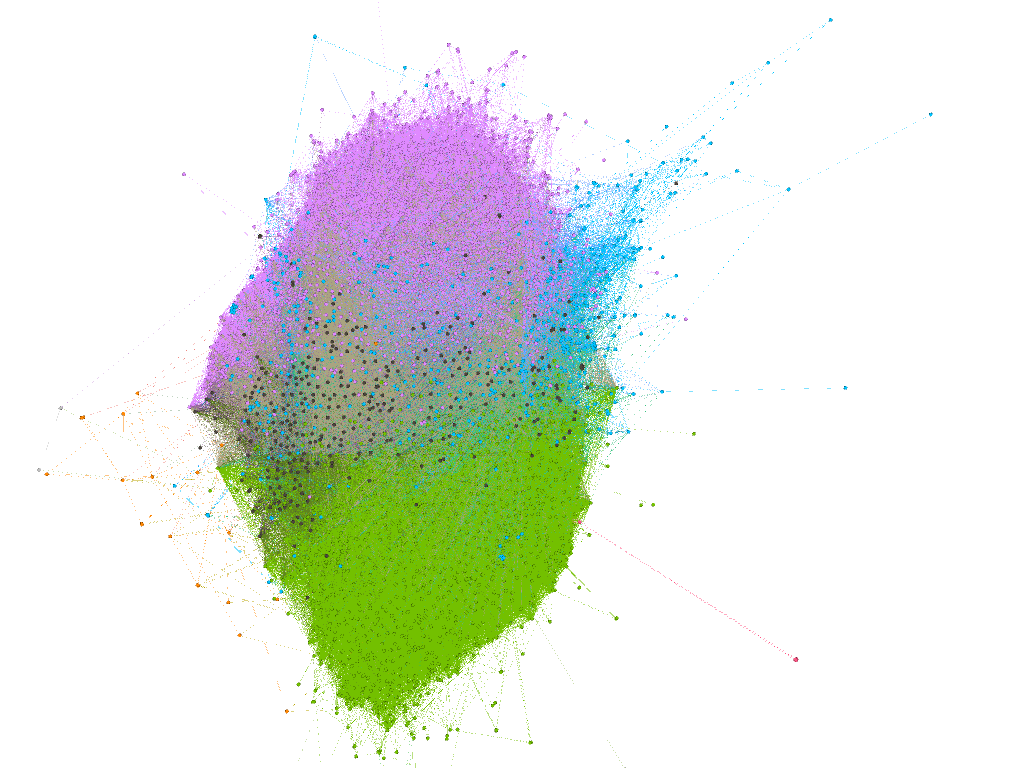
\includegraphics[width=\columnwidth]{graphics/atLeast1WorkCommunity.png}
	\caption{At least one work in common graph coloured by community.}
	\label{fig:graph1CommunityColoured}
	\end{center}
\end{figure}

\begin{figure}[!hbt]
	\begin{center}
	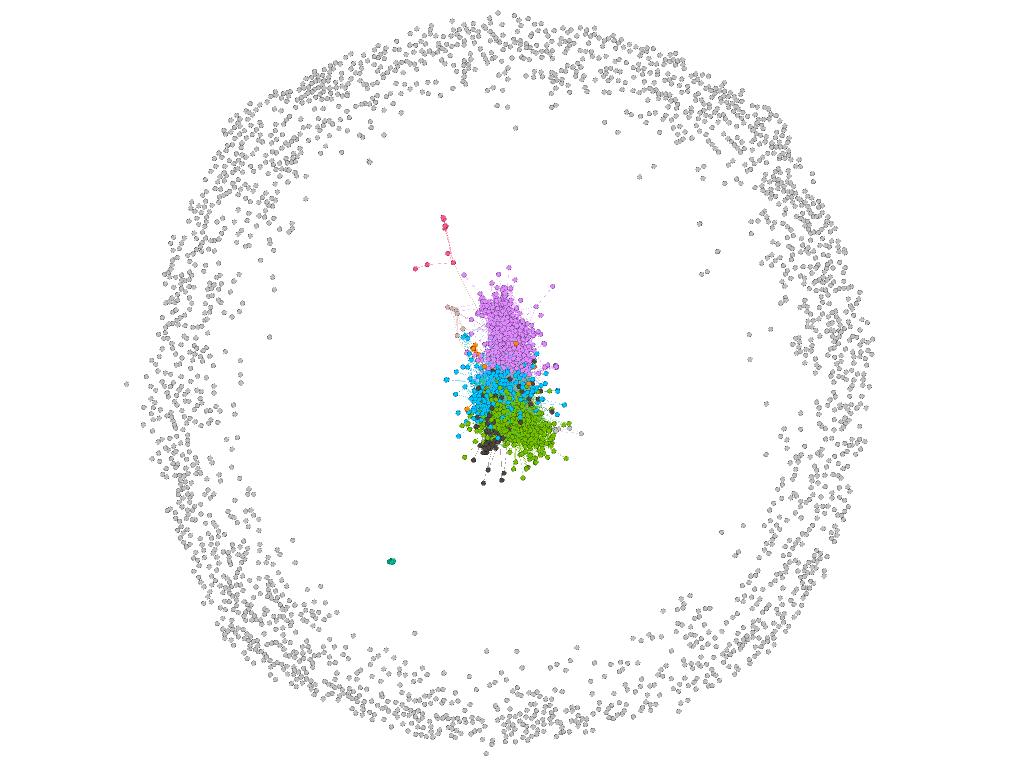
\includegraphics[width=\columnwidth]{graphics/atLeast10WorksCommunity.png}
	\caption{At least ten works in common graph coloured by community. Big cluster at the center, surrounded by loosely connected nodes.}
	\label{fig:graph10CommunityColoured}
	\end{center}
\end{figure}

Table~\ref{tab:graphComparision} shows metrics about each graph. Requiring more works in common decreases average degree circumstantially but doesn't change much modularity or network diameter.

\begin{table}[!hbt]
	\begin{center}
	\caption{Graph analysis}
	\label{tab:graphComparision}
	\begin{tabular}{|l|c|c|c|}
		\hline
		Graph & Avg Degree & Graph Density & Modularity \\
		\hline
		One work in common & 267 & 0.09 & 0.2 \\
		\hline
		Ten works in common & 9 & 0.003 & 0.29 \\
		\hline
	\end{tabular}\\
	\smallskip
	\begin{tabular}{|l|c|c|}
		\hline
		Graph & Network Diameter & Connected Components \\
		\hline
		One work in common & 6 & 18 \\
		\hline
		Ten works in common & 7 & 2261 \\
		\hline
	\end{tabular}
	\end{center}
\end{table}

\begin{figure}
	\centering
	\begin{subfigure}{.5\columnwidth}
		\centering
		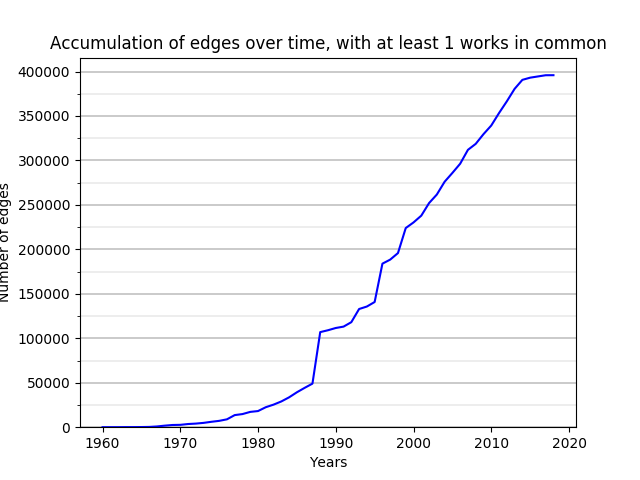
\includegraphics[scale=0.39]{graphics/accumulationEdges_1_1960-2018.png}
		\caption{At least one work in common}
		\label{fig:edgesOneWorkInCommon}
	\end{subfigure}%
	\begin{subfigure}{.5\columnwidth}
		\centering
		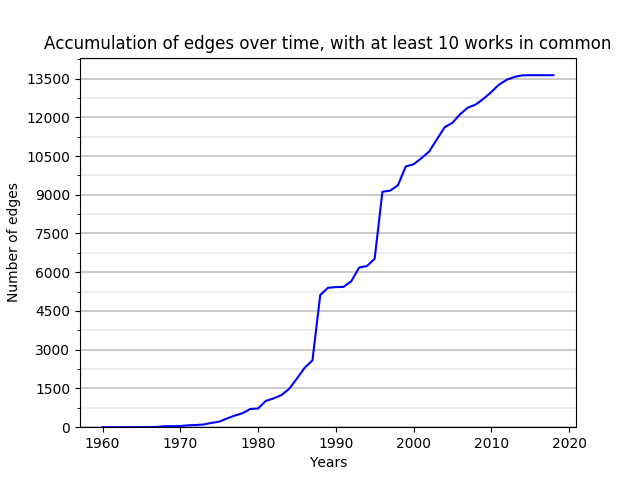
\includegraphics[scale=0.39]{graphics/accumulationEdges_10_1960-2018.png}
		\caption{At least ten works in common}
		\label{fig:edgesTenWorskInCommon}
	\end{subfigure}
	\caption{Grouwth of edges over time. For 1 and 10 works in common graphs}
	\label{fig:grouwthOfEdges}
\end{figure}

As proven by Fig.~\ref{fig:grouwthOfEdges} grouwth of edges by year follows a similar distribution regardless of how many works in common are used to build the social network.

\begin{figure}[!hbt]
	\begin{center}
	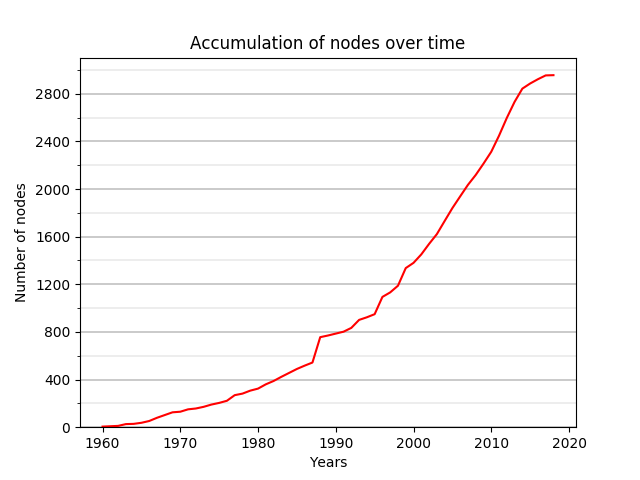
\includegraphics[width=\columnwidth]{graphics/nodesAccumulation.png}
	\caption{Grouwth of nodes over time.}
	\label{fig:grouwthOfNodes}
	\end{center}
\end{figure}
 
Fig.~\ref{fig:grouwthOfNodes} shows that more than half of the nodes are from last 18 years (2000 to 2018), giving us an idea of how much seiyuu industry is growing.

\FloatBarrier
Table~\ref{tab:top10atLeast1Work} shows top 10 nodes, for degree and betweenness centrality for "at least 1 work in common" definition. And Table~\ref{tab:top10atLeast10Works} does the same for "at least 10 works in common".

\begin{table}[!htb]
    \begin{minipage}{.5\textwidth}
        \centering
            \begin{tabular}{|l|c|}
				\hline
				Name & Degree \\ 
				\hline
				Takehito Koyasu & 1545 \\ 
				\hline
				Akira Ishida & 1488 \\ 
				\hline
				Mamiko Noto & 1422 \\ 
				\hline
				Nobuo Tobita & 1417 \\ 
				\hline
				Daisuke Namikawa & 1390 \\ 
				\hline
				Nobuyuki Hiyama & 1358 \\ 
				\hline
				Rikiya Koyama & 1331 \\ 
				\hline
				Jūrōta Kosugi & 1322 \\ 
				\hline
				Keiji Fujiwara & 1312 \\ 
				\hline
				Kazuhiko Inoue & 1309 \\ 
				\hline
			\end{tabular}
            \caption{Top 10 degree}
    \end{minipage}%
    \begin{minipage}{.6\textwidth}
        \centering
        \begin{tabular}{|l|c|}
				\hline
				Name & Betweenness Centrality \\
				\hline
				Takehito Koyasu & 49982.52 \\
				\hline
				Akira Ishida & 40221.50 \\
				\hline
				Daisuke Namikawa & 30448.43 \\
				\hline
				Nobuo Tobita & 29363.25 \\
				\hline
				Mamiko Noto & 29168.18 \\
				\hline
				Rie Kugimiya & 29122.31 \\
				\hline
				Miyuki Sawashiro & 28997.40 \\
				\hline
				Kazuhiko Inoue & 27693.88 \\
				\hline
				Daisuke Ono & 27034.592 \\
				\hline
				Keiji Fujiwara & 26802.69 \\
				\hline
		\end{tabular}
        \caption{Top 10 Betweenness centrality }
    \end{minipage}
    \caption{At least one work in common}
    \label{tab:top10atLeast1Work}
\end{table}

\begin{table}[!htb]
    \begin{minipage}{.5\textwidth}
        \centering
            \begin{tabular}{|l|c|}
				\hline
				Name & Degree \\
				\hline
				Takehito Koyasu & 311 \\
				\hline
				Akira Ishida & 273 \\
				\hline
				Mamiko Noto & 258 \\
				\hline
				Daisuke Namikawa & 232 \\
				\hline
				Katsuyuki Konishi & 229 \\
				\hline
				Keiji Fujiwara & 220 \\
				\hline
				Junichi Suwabe & 216 \\
				\hline
				Toshiyuki Morikawa & 215 \\
				\hline
				Rie Kugimiya & 213 \\
				\hline
				Nobuyuki Hiyama & 201 \\
				\hline
			\end{tabular}
            \caption{Top 10 degree}
    \end{minipage}%
    \begin{minipage}{.6\textwidth}
        \centering
        \begin{tabular}{|l|c|}
				\hline
				Name & Betweenness Centrality \\
				\hline
				Takehito Koyasu & 18489.44 \\
				\hline
				Mamiko Noto & 10988.96 \\
				\hline
				Daisuke Namikawa & 9570.48 \\
				\hline
				Akira Ishida & 8299.19 \\
				\hline
				Rie Kugimiya & 7560.16 \\
				\hline
				Katsuyuki Konishi & 7413.72 \\
				\hline
				Kenichi Ogata & 7160.54 \\
				\hline
				Harumi Sakurai & 6775.76 \\
				\hline
				Keiji Fujiwara & 5980.58 \\
				\hline
				Yoshimasa Hosoya & 5607.95 \\
				\hline
		\end{tabular}
        \caption{Top 10 Betweenness centrality }
    \end{minipage}
    \caption{At least ten works in common}
    \label{tab:top10atLeast10Works}
\end{table}

\section{Conclusion}
Both networks have fairly similar top 10s so it points to them having similar structure and connections amoung their nodes, aside from actual values.\\

From now on our definition for edges will be: \textit{at least 10 works in common, during the time frame between the first debut registered (1960) and the year of observation}. Because requiring more jobs in common means less amount of edges, this leaves a more understandable graph and we verified it does without changing its structure so much.\\

There's also other interesting definitions of relationship, for example we can use only common works from the last x years or from all time. This options weren't explored; having into account our limited time.\\

Table~\ref{tab:moreInfoSeiyuu} shows a little more information about seiyuu that appear on top 10s.
\begin{table}[!hbt]
	\begin{center}
	\caption{More information about seiyuu}
	\label{tab:moreInfoSeiyuu}
	\begin{tabular}{|l|c|c|c|c|}
		\hline
		Name & Popularity & Debut & Gender & Birthyear \\
		\hline
		Takehito Koyasu & 7235 & 1988 & Male & 1967 \\
		\hline
		Akira Ishida & 7612 & 1989 & Male & 1967 \\
		\hline
		Mamiko Noto & 7544 & 1988 & Female & 1980 \\
		\hline
		Daisuke Namikawa & 8304 & 1988 & Male & 1976 \\
		\hline
		Katsuyuki Konishi & 3702 & 1996 & Male & 1973 \\
		\hline
		Keiji Fujiwara & 2778 & 1986 & Male & 1964 \\
		\hline
		Junichi Suwabe & 10838 & 1996 & Male & 1972 \\
		\hline
		Toshiyuki Morikawa & 2455 & 1981 & Male & 1967 \\
		\hline
		Rie Kugimiya & 31668 & 1996 & Female & 1979 \\
		\hline
		Jun Fukuyama & 26811 & 1981 & Male & 1978 \\
		\hline
		Kenichi Ogata & 52 & 1974 & Male & 1942 \\
		\hline
		Harumi Sakurai & 341 & 2005 & Female & 1982 \\
		\hline
		Yoshimasa Hosoya & 4852 & 2006 & Male & 1982 \\
		\hline
		Nobuo Tobita & 139 & 1981 & Male & 1959 \\
		\hline
		Nobuyuki Hiyama & 1723 & 1988 & Male & 1967 \\
		\hline
		Rikiya Koyama & 2919 & 1996 & Male & 1963 \\
		\hline
		Jūrōta Kosugi & 114 & 1985 & Male & 1957 \\
		\hline
		Miyuki Sawashiro & 26501 & 1988 & Female & 1985 \\
		\hline
		Kazuhiko Inoue & 2445 & 1974 & Male & 1954 \\
		\hline
		Daisuke Ono & 24080 & 1996 & Male & 1978 \\
		\hline
	\end{tabular}
	\end{center}
\end{table}
